\subsection{Linear Regression}
Linear regression bases itself on the assumption of a linear relationship between the \textit{predictors} and the \textit{response}. 
Given a dataset of $p$ input variables (commonly called predictors), $X=[x_1, \, x_2, \, \ldots, \, x_p]$ and a dataset of output variables (commonly called the response) we seek a linear model on the form
\begin{equation}
\Tilde{y}=\hat{\beta_0}+\sum_{j=1}^{p}x_j\hat{\beta_j}.
\end{equation}
The scalar $\Tilde{y}$ is our prediction of the response, $\hat{\beta_0}$ the estimated intercept, and each $\hat{\beta_j}$ the estimated coefficient belonging to its corresponding predictor $x_j$. 

This equation is commonly written in vector form, 
\begin{equation}
\Tilde{\y}=\boldsymbol{X}^T\boldsymbol{\hat{\beta}},
\end{equation}

where given n different sets of input/output-variables, $\Tilde{\y}$ is the response-vector and $\boldsymbol{X}$ is a $n\times (p+1)$-matrix called the \textit{design matrix}. Here the $'+1'$ column in $\boldsymbol{X}$ is a row of ones for inclusion of the intercept in $\boldsymbol{\hat{\beta}}$, and the residual $p$ columns each of the p predictor variables. 


The ``true" model is assumed the form 
\begin{equation}\label{OG_y}
y=\beta_0+\sum_{j=1}^{p}x_j\beta_j+\epsilon,
\end{equation}
Our linear regression models are always estimations of the equation above, and we have no way of knowing the true $\boldsymbol{\beta}$. 
$\epsilon$ is some irreducible \textit{error-term} or \textit{residual-term} representing all variance in the data not explainable by the linear model; any variation due to randomness is included in this term. It is assumed $\epsilon \sim  
\mathcal{N}(0,\sigma^2)$, and given this assumption we get the expected value of $y_i$

\begin{equation}
    \fv{y_i} = \mathbf{X}_{i,*}\boldsymbol{\beta},
\end{equation}
and the variance of $y_i$
\begin{equation}
    \text{var}(y_i) = \sigma^2.
\end{equation}



Calculations are available in \hyperref[appendixB]{appendix B}.

\subsection{Cost- \& Loss-Functions}
The main objective when solving such a linear regression problem, is finding the optimal coefficients $\boldsymbol{\beta}$ that minimizes an error measure between $y_i$ and $\Tilde{y_i}$. 
What such an optimal solution evinces is dictated by the definition of our \textit{cost-function},  or \textit{loss-function}, which is simply metrics chosen to measure how much our predictions deviate from the "truth". 
A cost-function, $\text{Cost}(f,\mathcal{D} )$, is used to describe such a metric measuring a group of data-points, while a loss-function, $L(y, \hat{y})$, describes a metric regarding a single data-instance. 
The cost-function can be expressed in terms of the loss function
\begin{equation}
\text{Cost}(f,\mathcal{D}) = \frac{1}{n}\sum_{i=1}^n L(y_i, \hat{y_i}),
\end{equation}
as the average of the loss-function over the data. 
Through different choices of cost-function we end up with different methods for estimation, resulting in different models for the same data-set. 

%Depending on priorities when choosing, different models provide things like easier interpretation, lower \textit{bias}, or lower \textit{variance}. 

%https://www.baeldung.com/cs/cost-vs-loss-vs-objective-function


\subsection{Data handling}

\subsubsection{Scaling}\label{scaling}

In order for all predictors to have an equal starting point when training the model, it's often necessary to scale the data \citep[p. 398]{hastie}. Having one predictor with values of order $10^3$, and another predictor with values of order $10^{-3}$, the model could miss the predictive importance of the latter. Whether or not it is necessary to scale the data, depends on the choice of cost-function; Given two predictors of different magnitudes where the same relative change has equal impact on the response, the predictor of smaller magnitude would have coefficients of inversely proportional magnitude. If a cost-function penalizes bigger coefficients, as some does, the predictor of smaller magnitude would then be penalized more than it should. To alleviate the risk of such problems, it is thus necessary for many methods that we scale all data before training. 

A common choice for scaling is to use the \textit{standard scaler}. This method involves subtracting the mean and dividing by the standard deviation, for each feature respectively. Each of the columns will then have mean equal to zero and a standard deviation of one after the scaling. For the i-th datapoint and the j-th feature we get the transformation as indicated in Eq. \ref{standardize} \citep[Linear Regression]{morten}.

\begin{equation}\label{standardize}
    x_{ij} \rightarrow \frac{x_{ij}-\overline{x}_j}{\sigma_{x_j}}
\end{equation}

It's considered good practice to not scale the intercept, as it represents a constant term without variability and scaling it would worst case defeat it's purpose or worsen it's performance. It can be taken out during training and later be recalculated as Eq. \ref{bet0} shows \citep[Resampling methods]{morten}. We will see later how some methods would produce different results if a scaled intercept was included in the training. Taking out the intercept amounts to removing the column of 1's in the design matrix. 

\begin{equation}\label{bet0}
    \beta_0 = \frac{1}{n}\sum_{i=0}^{n-1}y_i - \frac{1}{n}\sum_{i=0}^{n-1}\sum_{j=1}^{p-1}X_{ij}\beta_j
\end{equation}

\subsubsection{Splitting data into sets}\label{overfitting}

When training a model we want it to learn the underlying pattern of the data that is (hopefully) representative for the entire population the data is sampled from. 
Testing a model on the same data it's trained on could give a false impression of it's accuracy; a model that takes into account variation specific to the data it's trained on (that's not representative for the larger population) would get rewarded in this testing, while a model that does not take it into account would get punished. 

We therefore need (at least) two datasets; a set used for training and a set used for testing, to give us a more impartial evaluation of the model. The two datasets are named respectively "training data" and "test data". As can be inferred by the names, we use the training data in the training (or \textit{fitting}) of the model, while the test set is used to evaluate the performance of our final chosen model. 
Additionally one can choose to include a "validation" set in the split; this validation set would then be applied in the model selection phase.

An important concept in train-test splitting is to \textbf{never} touch the test-set before the final evaluation. The test-set is supposed to act as never-before seen data for the model, and given a limited data set it's the closest one gets to an impartial assessment. 
If using a scaler, fitting of the scaler should be done after the split and solely on the training data - and this scaler, fit to the training data, then applied to the test data when testing. 

Splitting data is an important tool to help avoid \textit{overfitting} and \textit{underfitting} of the model, and ensure a more generalizable fit. Overfitting and underfitting is elaborated further in  section G; "\textit{Bias-Variance Tradeoff}".
\julie{KILDER}
% We will use the latter to understand when the model starts learning beyond the underlying pattern. At this point, the training should be stopped. The test data is used for model selection.

% If we develop a too complex model that gets specialized to the training data and perhaps even noise, we get a case of \textit{overfitting}. 

% In practice, we look at the error rate of the training and test data. The error on the training data will continue to decrease. For the test data, we will initially see a decrease in the error. After some time of training, this will increase again. At this point, the model is overfitting to the training data and we have our stopping criteria.

%\plothere{Plot here of loss on training and test data to explain overfitting, as in Hastie}

% \begin{figure}[h!]
% \centering
% 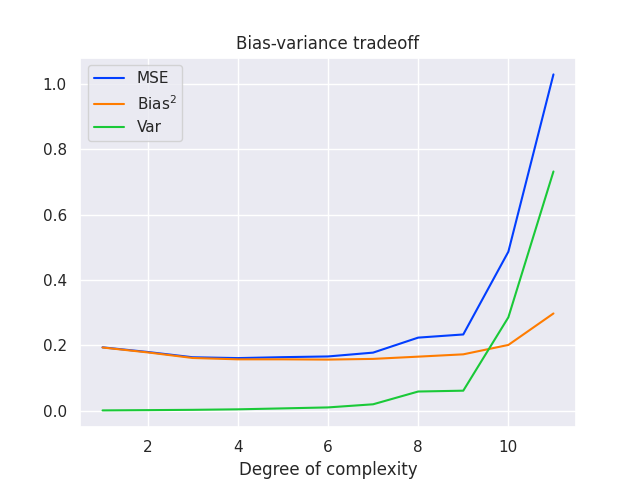
\includegraphics[width=1\linewidth]{project_1/figures/bias_var_bootstrap.png}\label{plot_overfit}
% \caption{\mia{must insert the correct image}}
% \label{train_test_overfit}
% \end{figure}



%\subsubsection{Error estimation}

%The metric we truly want is the loss on independent data not seen or used in any way during training. Although the test data has not been trained on, we have used it to decide on when to stop the training. Our model is therefore not completely independent of the test data. Ideally one could have separated the data into three sets to overcome this. This is necessary to correctly choose between models, but only two sets are needed for training. The three datasets are typically called "training data", "validation data" and "test data". \mia{cite for paragraph}

%\julie{Du må hjelpe meg her, Julie $\downarrow$}

%The error measure we truly want is the prediction error on an independent test data set $\tau$: 
%\begin{equation}\label{error_test}
    %\text{Error}_{\tau} = \fv{L(\y,\hat{f}(\boldsymbol{x})) | \tau}
%\end{equation}

%The training error is not a good estimate of this. As explained in sec. \ref{overfitting} we can overfit to decrease this error measure. The training error is expressed as: 

%\begin{equation}
    %\overline{\text{err}} = \frac{1}{n}\sum_{i=0}^{n-1} L(y_i, \Tilde{y}_i)
%\end{equation} 

%\julie{Du må hjelpe meg her, Julie $\uparrow$}

\subsection{Resampling methods}

Generally, we want as much data as possible for the training of a model. When holding off some of the data for testing, we lose this data for training. It's therefore of interest to explore methods that allow for a train-test split of the data, while still keeping as much data as possible for training. 

\subsubsection{K-fold cross-validation}
\textit{K-fold cross-validation} is one such resampling method. The $K$ represents a number that must be chosen by the developer as they see fit. We divide our dataset into $K$ parts $\mathcal{F}_k$, called folds. $K-1$ folds are used as training data, while the remaining fold is used as test data. The model trained when the $k$-th fold is held out, is denoted $f^{k}$. 
The procedure is repeated $K$ times, holding out a new fold each time. For k-fold cross-validation we get an estimated error as the mean of the $K$ test errors as shown in Eq. \ref{cv}. \citep[p. 241]{hastie}


\begin{equation}\label{cv}
    CV_{error} = \frac{1}{K} \sum_{k=1}^{K} \frac{1}{|\mathcal{F}_k|} \sum_{i \in \mathcal{F}_k} L\left(y_i, f^{k}({x}_i)\right) 
\end{equation}

There is both advantages and disadvantages of this method. The maifor a high $K$ it is quite computationally costly. Another disadvantage is that there is no clear choice of $K$. There is a trade-off between bias and variance. A smaller K leads to lower variance, but higher bias. On the other side, a higher K leads to low bias, but high variance. The extreme case of the ladder is leave-out-one cross-validation (LOOCV), where every datapoint acts as a fold. It will lead to an unbiased error measure, but the variance will be quite large \citep[p. 242]{hastie}.

On the other hand an advantage of cross-validation is having a bigger training set, while maintaining  is left for training. Another advantage is that the estimated error (Eq. \ref{cv}) will be closer to the true generalization error measure. This is a consequence of the error being averaged over many different models, and thereby to higher degree taking into account randomness associated with data-selection. \mia{cite}

\julie{se over siste setningene igjen}

\subsubsection{Bootstrapping}
Bootstrapping is a method where we draw with replacement from the original data to have a new data set for training. Every bootstrap sample should have the same size as the original data set, $n$. We generate many such samples and repeat the training. The total number of samples is denoted by B. This is meant to simulate new experiments.\mia{cite} 
For the b-th bootstrap sample we obtain model $\hat{f}_b$ \citep[p. 249]{hastie}.

The error could calculated as the mean of the error:

\begin{equation}
    BS_{error} = \frac{1}{n}\frac{1}{B}\sum_{i=0}^{n-1}\sum_{b=1}^{B} L\left(y_i, \hat{f}_b(x_i)\right)
\end{equation}

\mia{more}

%\begin{equation}
%    \widehat{\text{Err}}^{(1)} = \frac{1}{n} \sum_{i=0}^{n-1} \frac{1}{|C_{[-i]}|} \sum_{b \in C_{[-i]}} L\left(y_i; \hat{f}_b(x_i)\right)
%\end{equation}

%However, this might be too optimistic. On average we have 63.2\% of the original observations in a bootstrap sample. This corresponds to 36.8\% not being in the bootstrap sample at all. \mia{more} This correct error measure for bootstrapping is therefore \citep[p. 251]{hastie}: 

%\begin{equation}
    %BS_{error} = 0.368 \overline{\text{err}} + 0.632 \widehat{\text{Err}}^{(1)}
%\end{equation}


\subsection{Ordinary least squares}

Ordinary least squares is a linear regression method where we seek to minimize the following cost function:

\begin{equation}\label{cost_ols}
    C(\bet) = \frac{1}{n}\sum_{i=0}^{n-1}(y_i-\Tilde{y}_i)^2
\end{equation}

From Eq. \ref{cost_ols} we can derive the equation for the optimal $\bet$. This is done by taking the derivate of the cost function wrt. $\bet$ and finding the minimum. The optimal $\bet$ in OLS is shown in Eq. \ref{betaols}. 

\begin{equation}\label{betaols}
    \hat{\bet}_{\text{OLS}} = \betta = \boldsymbol{H}\y
\end{equation}

The $\boldsymbol{H}$ is popularly called the Hessian matrix. The Hessian matrix for OLS specifically is stated in Eq. \ref{betaols}, but the term "Hessian matrix" can be used for any linear regression method.


Ordinary least squares provide an unbiased estimation - meaning the expected distance between our prediction and the truth is zero. 

\begin{equation}
    \fv{\hat{\bet}_{OLS}} = \bet
\end{equation}

\begin{equation}
   \text{var}(\hat{\bet_{OLS}}) = \sigma^2 (\mathbf{X}^T\mathbf{X})^{-1}
\end{equation}

OLS regression is invariant to the scaling of the data.

%\mia{Could discuss a bit the advantages and disadvantages of the two compared to each other. Ridge best for prediction, lasso best for model selection. Could link to AIC and BIC, but probably just messy to include to more measures. Could discuss that we could have methods that are combinations of the two $\rightarrow$ elastic net. There is no gradient for lasso, but there is for ridge. Must mention here or somewhere else that it is especially important to scale when we have a penalty because the penalty is not scale invariant.}

%\mia{I think it could be useful with some figures in the theory, showing bias, variance, the scaling of the parameters in ride and lasso, etc. Could use either size of beta against lambda or the geometric variant. }

\subsection{Penalized linear regression methods}

An extension of the ordinary least squares method is to add a penalization term. A general term for this is shrinkage methods. There are many reasons why this is often preferred. \mia{cite for the last statement}

Firstly, to perform OLS we assume that the matrix $\boldsymbol{X}^T\boldsymbol{X}$ in Eq. \ref{betaols} is invertible. This may not always be the case due to correlation between the predictors in the data set or if $p > n$. Then the matrix will not be full rank. 

A mathematical fix to this is to add a (small) number along the diagonal: 
\begin{equation}\label{pen}
    \bet = (\mathbf{X}^T\mathbf{X}- \lambda\boldsymbol{I})^{-1}\mathbf{X}^T\mathbf{y}
\end{equation}

Secondly, these methods also reduce overfitting. \mia{cite (Morten)}

Eq. \ref{pen} is the general equation for penalized regression. The parameter $\lambda$ controls the regularization. Furthermore, we have different types of penalties. Two types are the L1-norm penalty, also known as Lasso, and the L2-norm penalty, known as Ridge. We will see that different types of penalties give different properties and interpretations.

\subsubsection{Ridge Regression}\label{ridge_sec}

In Ridge regression, an L2-norm penalty is used. This amounts to the following cost-function (Eq. \ref{ridge}) and constraint on the $\beta$'s (Eq. \ref{ridge_constraint}):

\begin{equation}\label{ridge}
     C(\bet) = \frac{1}{n} \sum_{i=0}^{n-1} \left( y_i - \sum_{j=1}^{p-1} X_{ij}\beta_j \right)^2 + \lambda\sum_{j=1}^{p-1} \beta_j^2 
\end{equation}



\begin{equation}\label{ridge_constraint}
    \sum_{j=1}^p \beta_j^2 \leq t, 
\end{equation}

The value of t is directly related to the value of $\lambda$ \citep[p. 63]{hastie}.

The solutions produced by Ridge regression depend on the scaling of the data. It is therefore especially important to standardize the data as explained in sec. \ref{scaling}. Ridge regression puts a penalty on all the $\beta$-terms except the intercept which is held out during training. If it had been included, the model would depend on the chosen origin \citep[p. 63]{hastie}.
The value of $\beta_0$ is later calculated as Eq. \ref{bet0} shoes. 

In ridge regression, the values of $\beta_j$ are forced closer to zero, but can never be zero completely. \mia{consequences}

It can be showed that $\bet_{OLS}$ and $\bet_{Ridge}$ are related as shown in Eq. \ref{ridgeOLS}. 

\begin{equation}\label{ridgeOLS}
    \bet_{Ridge} = \frac{1}{1+\lambda}\bet_{OLS}
\end{equation}




\subsubsection{Lasso Regression}

Lasso regression is another shrinkage method. This method uses an L1-norm penalty. We get the cost function and constraint on $\beta$ as Eq. \ref{lasso} and Eq. \ref{lasso_constraint} respectively shows. 

\begin{equation}\label{lasso}
     C(\bet) = \frac{1}{n} \sum_{i=0}^{n-1} \left( y_i - \sum_{j=0}^{p-1} X_{ij}\beta_j \right)^2 + \lambda\sum_{j=0}^{p-1} |\beta_j|
\end{equation}

\begin{equation}\label{lasso_constraint}
    \sum_{j=1}^p | \beta_j | \leq t, 
\end{equation}


The value of t is directly related to the value of $\lambda$ \citep[p. 68]{hastie}.


As in Ridge regression, the intercept is held out. The same reasoning holds for Lasso regression and the reader is refereed to sec. \ref{ridge_sec}.

In Lasso regression the value of the $\beta$'s can be out to zero. If the value of $\lambda$ is suffeciently large, we will see that more coefficients become zero. Lasso is therefore also also a method for feature selection. 

%\subsubsection{Comparison}

%\plothere{Sirkel og diamant}

\subsection{Bias-Variance Tradeoff}

\julie{JULIE}

\subsubsection{Bias}
The bias of an estimator is the difference between the expected value of the estimator and its true value as shown in Eq. \ref{bias}. 

\begin{equation}\label{bias}
    \text{Bias}(\hat{\bet}) = \fv{\hat{\bet}}-\bet
\end{equation}

The bias is the distance between the actual target and the prediction. If a model is overfitted the bias is low. The predictions are very close to the target in the training data set. An underfitted model however, has a high bias. In both cases, we have a model that does not capture the real underlying pattern but is rather too complex or simple respectively. High bias entails a systematic miss of the true pattern in the data. %It can easily be understood by looking at an archery target \plothere{Add a figure after variance and explain all}. 

\subsubsection{Variance}

The variance of an estimator is its sensitivity to fluctuations in the data sets. If the predictions vary a lot depending on which data set we train on, it has high variance. The equation for the calculation of the quantity is shown in Eq. \ref{var}. 

\begin{equation}\label{var}
    \text{Var}(\hat{\bet}) = \fv{\hat{\bet}-\fv{\hat{\bet}}^2} = \fv{\hat{\bet}^2} - \fv{\hat{\bet}}^2
\end{equation}

An overfitted model generally has high variance. As the model learns the specific training data and not the underlying pattern, it is reasonable that the model becomes very sensitive to the specific data it is tested on.

\subsubsection{The trade-off}

%\mia{mention that we here use OLS, but that the concepts hold in general}

During training the objective is to minimize the cost function.  We can decompose the expression for the expected error for a model fit with ordinary least squares (OLS) regression. Calculations are available in \hyperref[appendixB]{appendix B}.

\begin{equation}\label{biasvar}
    \fv{(\y - \yt)^2} = \text{Bias}(\yt)^2 + \text{var}(\yt) + \sigma^2
\end{equation}

Eq. \ref{biasvar} shows how the expected error is decomposed into a bias term, a variance term, and an irreducible error. The latter comes from $\epsilon$ in Eq. \ref{OG_y}. As the term irreducible error suggests, there is nothing for us to do with this term. We are therefore left with a bias term and a variance term. These terms are inversely related and in our to have the smallest error in total, we need to balance them. 

An overfitted model has low bias, but high variance. An underfitted model has the opposite, high bias and low variance. In fig. \ref{train_test_overfit} this corresponds to high bias and low variance in to the left and the opposite to the right. The figure furthermore shows how there is a sweat-spot where the trade-off between the two gives the lowest possible MSE.


\subsection{Evaluation measures}

The \emph{mean squared error} (MSE) is defined as: 

\begin{equation}\label{mse}
    \text{MSE} = \frac{1}{n}\sum_{i=0}^{n-1}(y_i-\Tilde{y}_i)^2
\end{equation}

The number of data points in our training data is $n$ while the prediction for the i-th data point is denoted $\Tilde{y}_i$. MSE is a popular error measure for linear regression models. 

We see how the OLS regression method is inherently designed to minimize MSE.

\begin{equation}
    R^2 = 1 - \frac{RSS}{TSS}= 1 - \frac{\sum_{i=0}^{n-1}(y_i-\Tilde{y}_i)^2}{\sum_{i=0}^{n-1}(y_i-\overline{y}_i)^2}
\end{equation}

$R^2$ is a measure of how much of the variance in the data the model explains. %\mia{cite} 
Furthermore $R^2 \in [0,1]$. If $R^2 = 1$ the model perfectly explains all variance, whereas a value of 0 would mean does not explain any of the variance. The numerator is the sum of the squared residuals, also called RSS. The denominator is the total sum of squares, in short TSS. \mia{cite}

